
\chapter{Simulação em hardware}

Com o objectivo de simular 


\section{Micro-controladores}

\subsection{Arduino Nano}

dataset 



\begin{figure}[!tbp]
	\centering
	\begin{minipage}[b]{0.4\textwidth}
		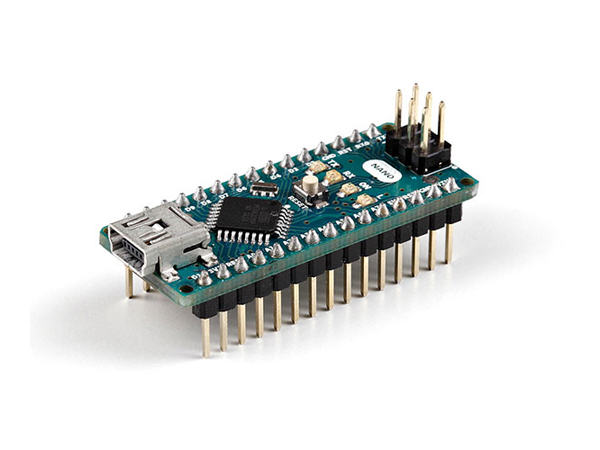
\includegraphics[width=\textwidth]{img/hardware/nano-img.jpg}
		\caption{Flower one.}
	\end{minipage}
	\hfill
	\begin{minipage}[b]{0.4\textwidth}
		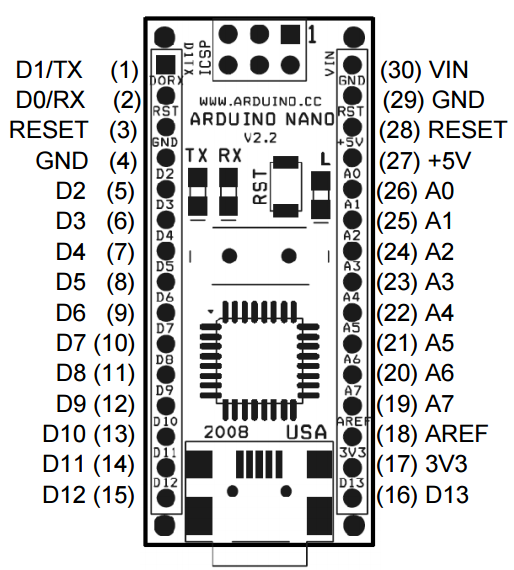
\includegraphics[width=\textwidth]{img/hardware/nano-esquema.png}
		\caption{Flower two.}
	\end{minipage}
\end{figure}





\subsection{Raspberry pi }


\section{Sensores}

\subsection{Sensor de temperatura (TTC 104)}

\begin{figure}[!tbp]
	\centering
	\begin{minipage}[b]{0.4\textwidth}
		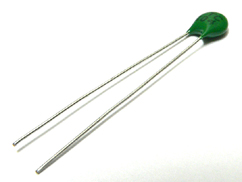
\includegraphics[width=\textwidth]{img/hardware/temperatura.jpg}
		\caption{Flower one.}
	\end{minipage}
	\hfill
	\begin{minipage}[b]{0.4\textwidth}
		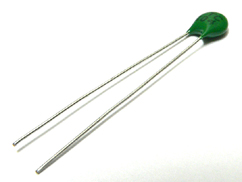
\includegraphics[width=\textwidth]{img/hardware/temperatura.jpg}
		\caption{Flower two.}
	\end{minipage}
\end{figure}



\begin{table}[]
	\centering
	
	\begin{tabular}{|
		>{\columncolor[HTML]{C0C0C0}}c |c|} \hline
		Resistencia & isso \\ \hline
		Valor máximo & isso \\ \hline
		Valor minimo & isso \\ \hline
		Nome & isso \\ \hline
	\end{tabular}
	\caption{Características do sensor TTC 104}
	\label{my-label}
\end{table}





\newpage

\subsection{Sensor de luminosidade (GL5528)}

\begin{figure}[!tbp]
	\centering
	\begin{minipage}[b]{0.4\textwidth}
		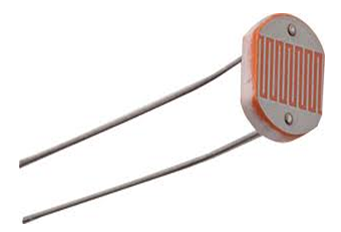
\includegraphics[width=\textwidth]{img/hardware/luminosidade.png}
		\caption{Flower one.}
	\end{minipage}
	\hfill
	\begin{minipage}[b]{0.4\textwidth}
		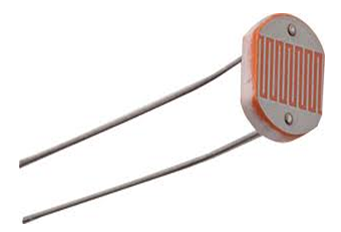
\includegraphics[width=\textwidth]{img/hardware/luminosidade.png}
		\caption{Flower two.}
	\end{minipage}
\end{figure}



\begin{table}[]
	\centering
	
	\begin{tabular}{|
			>{\columncolor[HTML]{C0C0C0}}c |c|} \hline
		Resistencia & isso \\ \hline
		Valor máximo & isso \\ \hline
		Valor minimo & isso \\ \hline
		Nome & isso \\ \hline
	\end{tabular}
	\caption{Características do sensor GL5528}
	\label{my-label}
\end{table}


\subsection{Sensor de nível líquido}

\begin{figure}[!tbp]
	\centering
	\begin{minipage}[b]{0.4\textwidth}
		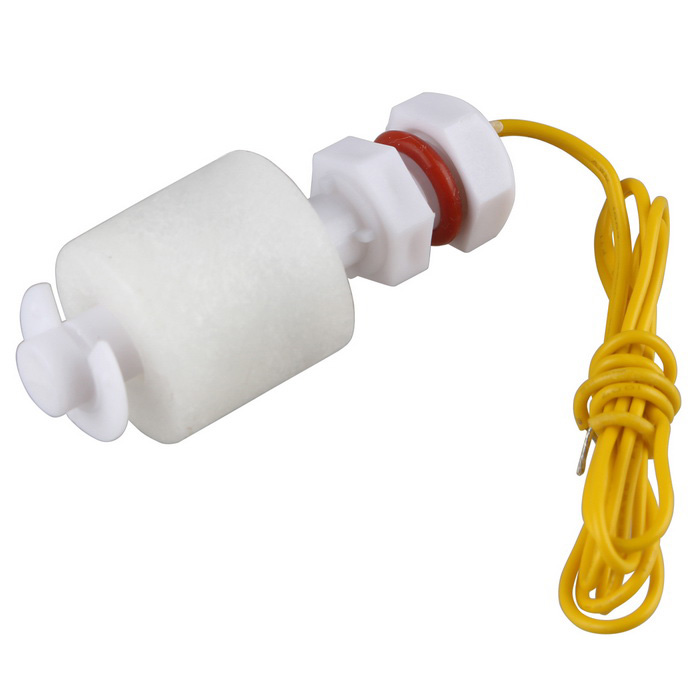
\includegraphics[width=\textwidth]{img/hardware/liquido.JPG}
		\caption{Flower one.}
	\end{minipage}
	\hfill
	\begin{minipage}[b]{0.4\textwidth}
		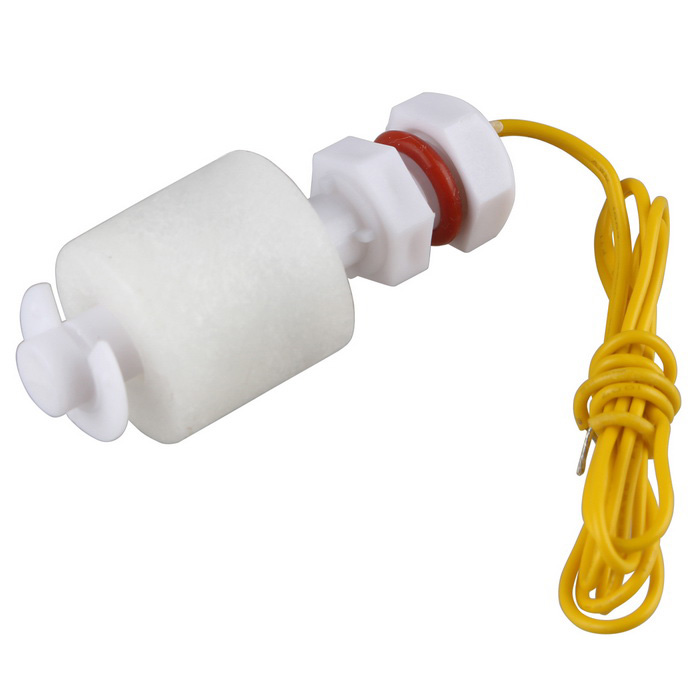
\includegraphics[width=\textwidth]{img/hardware/liquido.JPG}
		\caption{Flower two.}
	\end{minipage}
\end{figure}


\subsection{Simulador de bomba para transferências de águas (led)}

\begin{figure}[!tbp]
	\centering
	\begin{minipage}[b]{0.4\textwidth}
		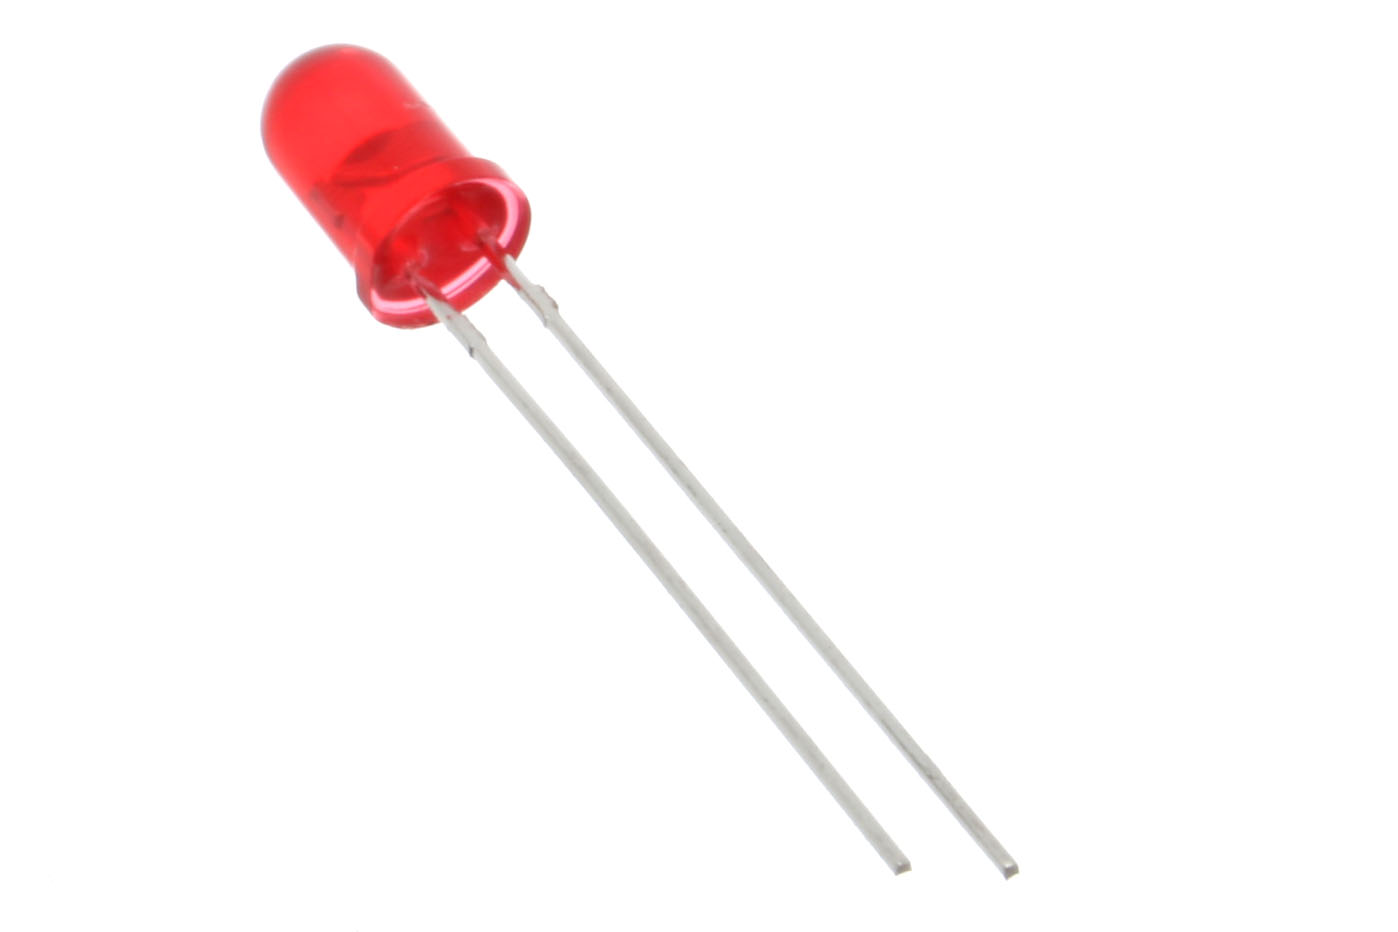
\includegraphics[width=\textwidth]{img/hardware/led.jpg}
		\caption{Flower one.}
	\end{minipage}
	\hfill
	\begin{minipage}[b]{0.4\textwidth}
		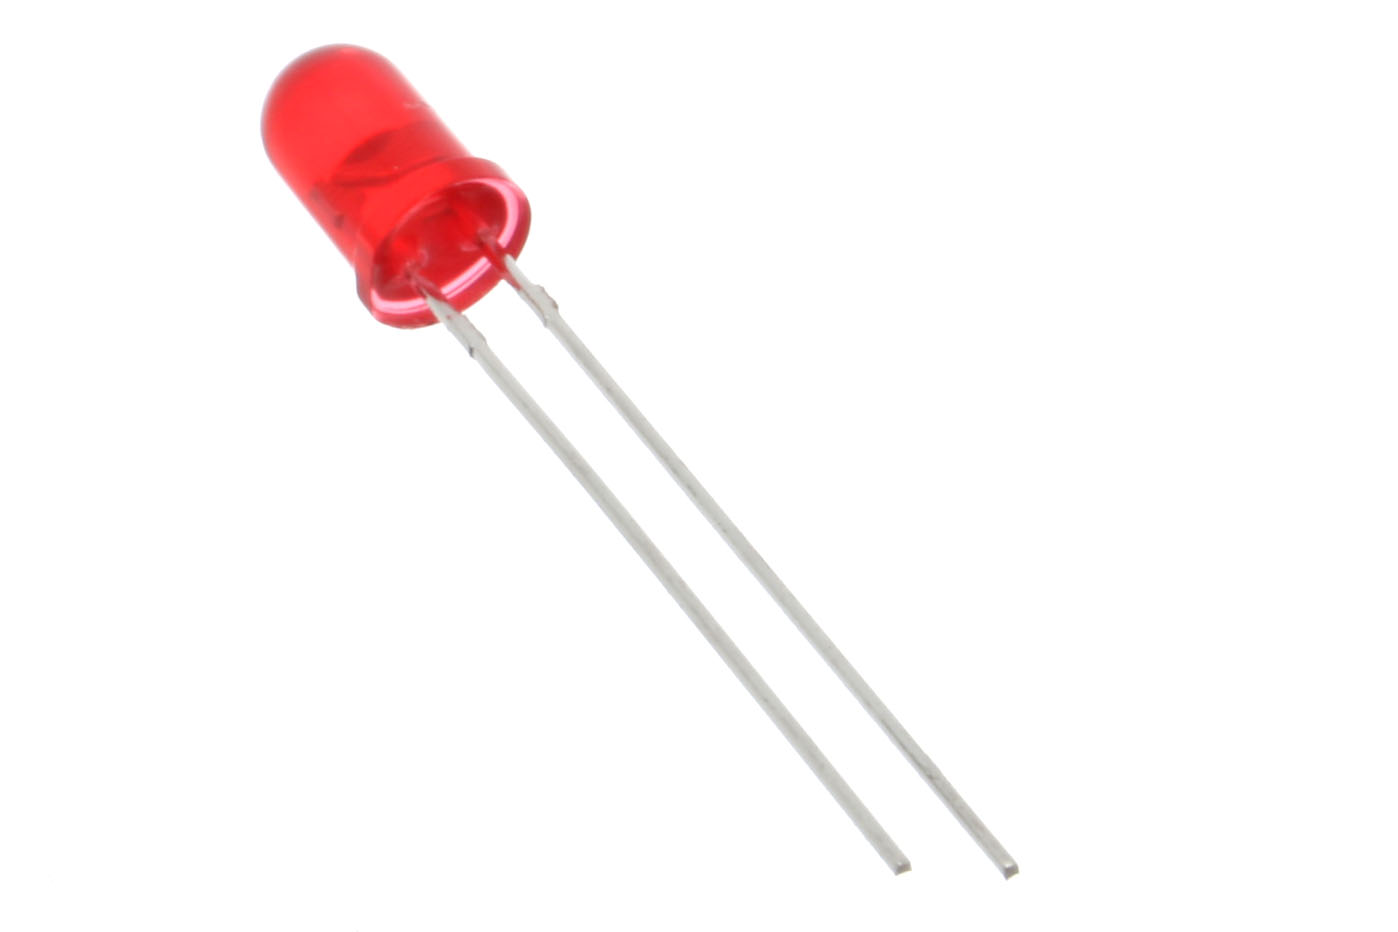
\includegraphics[width=\textwidth]{img/hardware/led.jpg}
		\caption{Flower two.}
	\end{minipage}
\end{figure}


\section{Comunicação}



\section{Interligação de componentes}


